\section{Introduction}
	Wireless sensor network \cite{wsn} is a popular area for research now days, due to vast potential usage of sensor networks in different areas.A sensor network is a comprised of sensing, processing, communication ability which helps to observe, instrument,react to events and phenomena in a specified environment \cite{wsn2} \cite{wsn3}.This kind of network  enables  to  connect  the  physical  world  to  environment.   By  networking
	tiny sensor nodes, it becomes easy to obtain the data about physical phenomena which was very much difficult with conventional ways.Wireless sensor network typically consist of tens to thousands of nodes. These nodes collect, process and cooperatively  pass  this  collected  information  to  a  central  location.   WSNs  have unique characteristics such as low duty cycle, power constraints and limited battery  life,  redundant  data acquisition,  heterogeneity  of  sensor  nodes,  mobility  of nodes,  and  dynamic  network  topology,  etc  \cite{wsn2}. 
\section{Application Of WSN}
	There are numerous applications of WSNs in Military, traffic monitoring and control, medical device monitoring and in many other areas. Some of applications are discussed below:
	\begin{figure}
	\subsection{Military or Border Surveillance Applications}
		WSNs are becoming an integral part of military command,control,communicatio and intelligence systems.Sensors can be deployed in a battle field to
		monitor the presence of forces and vehicles, and track their movements, enabling close surveillance of opposing forces  see \ref{fig:x army} .\cite{application}
	
	%Figure Army Application Right Here
	%	\begin{figure}[h!]
	%		\centering
	%		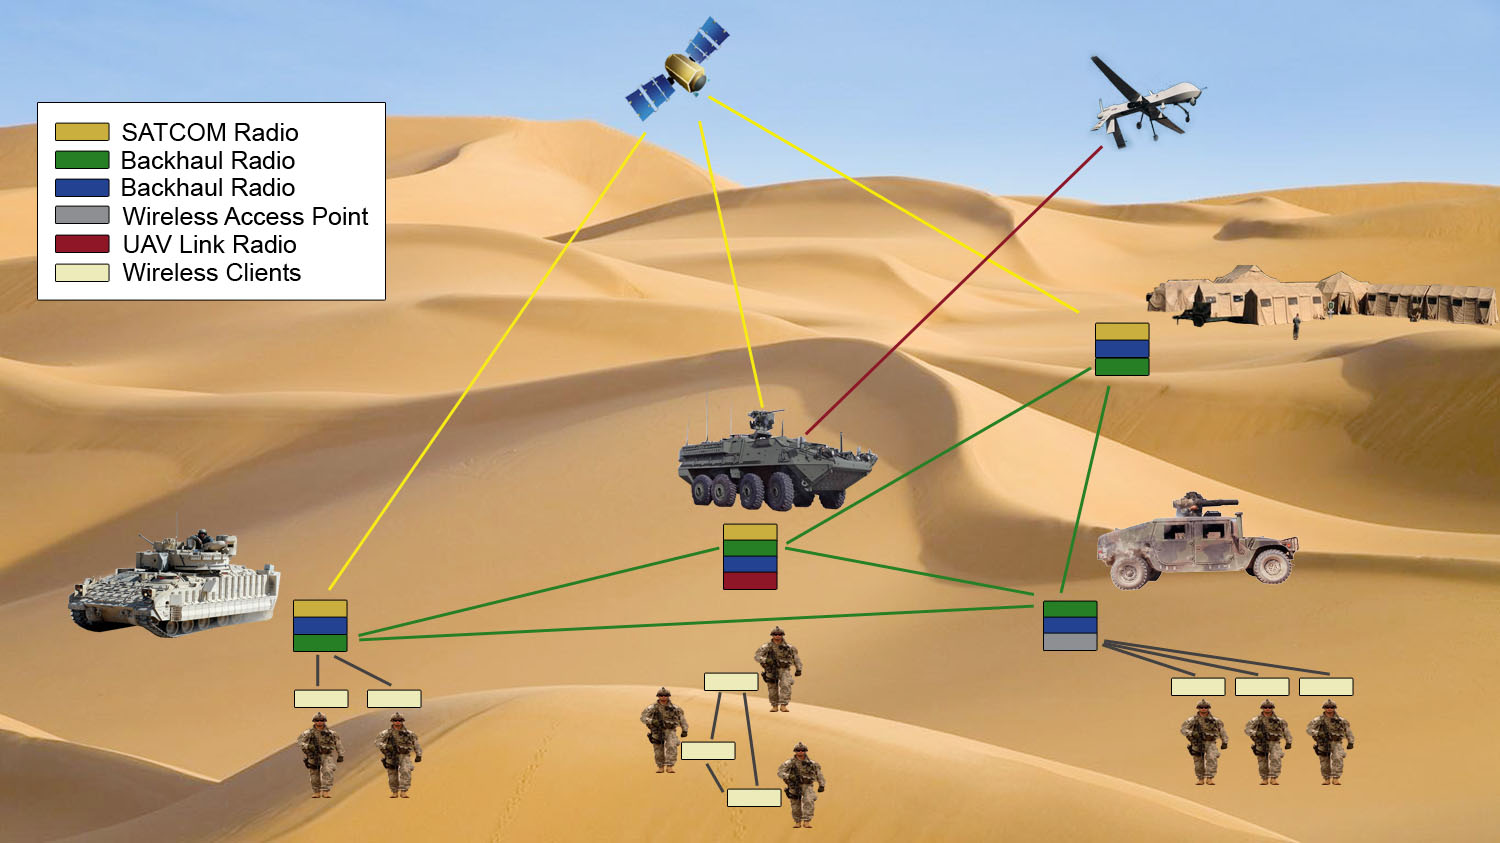
\includegraphics[scale=0.5,width=15cm,height=9cm]{photos/army.jpg}
	%		\caption{Military Surveillance App}
	%		\label{fig:x army}

	%	\end{figure}
	
	\hfill
	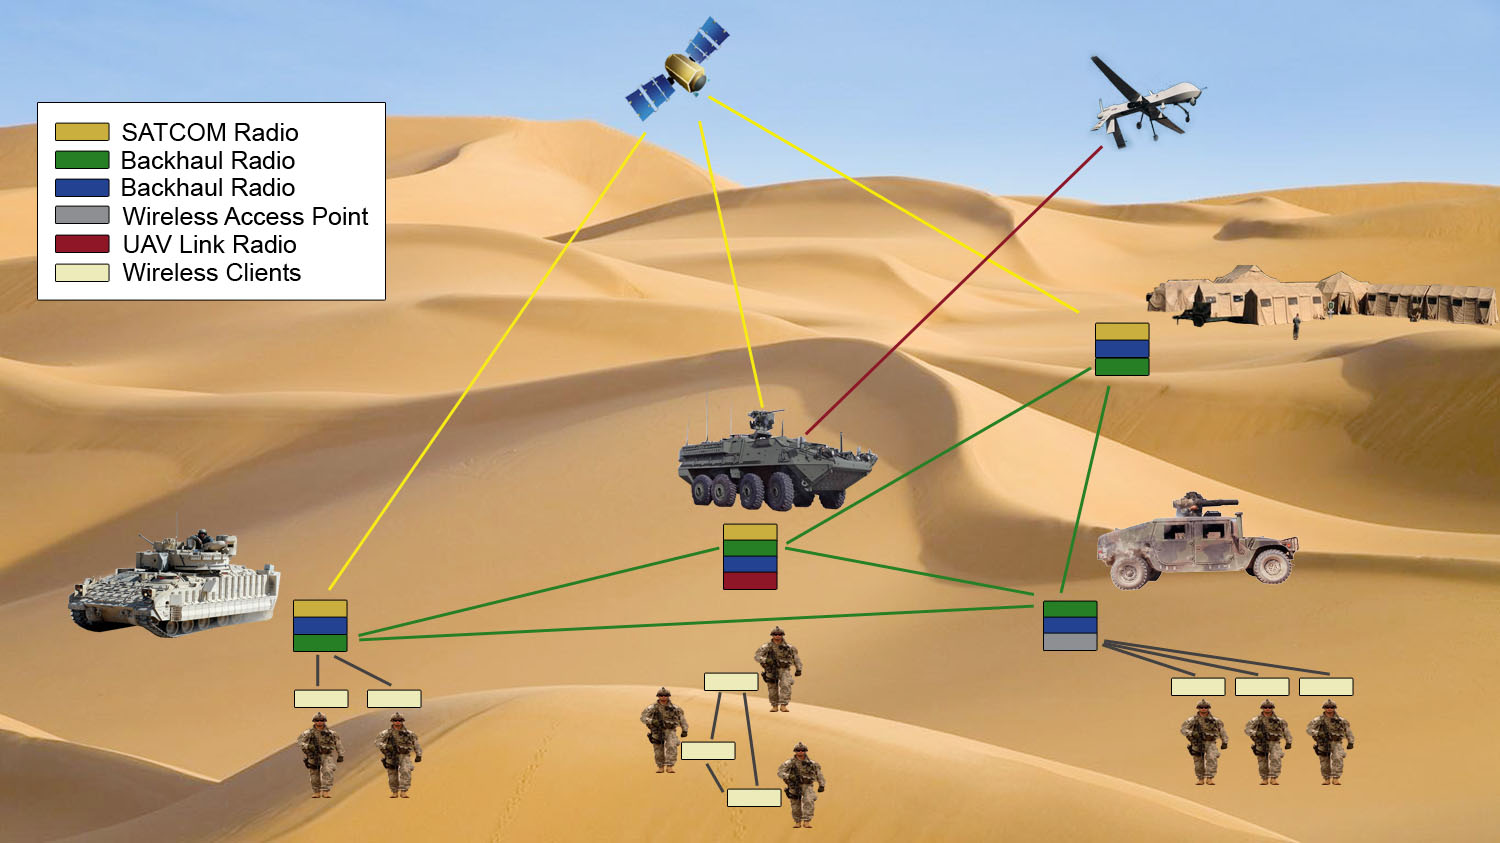
\includegraphics[scale=0.5,width=12cm,height=6.5cm]{photos/army.jpg}
	\caption{Military Surveillance App}
	\label{fig:x army}
		\centering
	\hspace*{\fill}
	\end{figure}

	\begin{figure}
	\subsection{Environmental Conditions Monitoring}
		 WSN applications in this area include monitoring the environmental conditions affecting crops or livestock,monitoring  temperature,  humidity  and lighting  in  office buildings, and so on. These monitoring modules could even be  combined  with  actuator modules which can control,for example , the amount of fertilizer in the soil, or the amount of cooling or heating in a building, based on distributed sensor measurements\cite{application} see\ref{fig:x Environmental_Conditions_Monitoring}.

	
	%Figure Env Condition Monitoring Right here
	%\begin{figure}[h!]
	%	\centering
	%	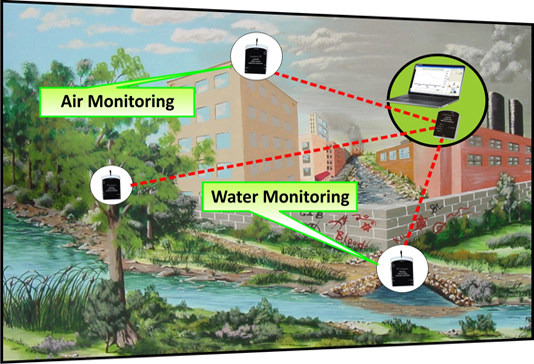
\includegraphics[scale=0.5,width=15cm,height=9cm]{photos/env.jpg}
	%	\caption{Environmental Conditions Monitoring}
	%	\label{fig:x Environmental_Conditions_Monitoring}	
	%\end{figure}

	
	\hfill
	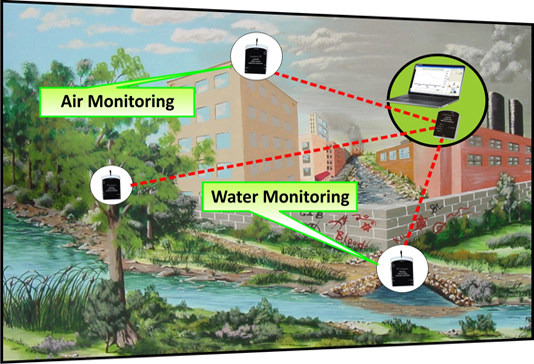
\includegraphics[scale=0.5,width=12cm,height=6.5cm]{photos/env.jpg}
	\caption{Environmental Conditions Monitoring}
		\centering
	\label{fig:x Environmental_Conditions_Monitoring}
	\hspace*{\fill}
 	\end{figure}

	\begin{figure}
	\subsection{Health Care Applications}
		Wireless  sensor  networks  can  be  used  to  monitor  and track  elders  and  patients  for  health  care  purposes,  which can significantly relieve the severe shortage of health care personnel  and  reduce  the  health  care  expenditures  in  the current  health  care  systems.  For  example  sensors  can  be deployed in a patient’s home to monitor the behaviors  of the patient. It can alert doctors when the patient falls and requires immediate medical attention\cite{application} see \ref{fig:x Health_Care_Applications}.
		
		
		
		\hfill
		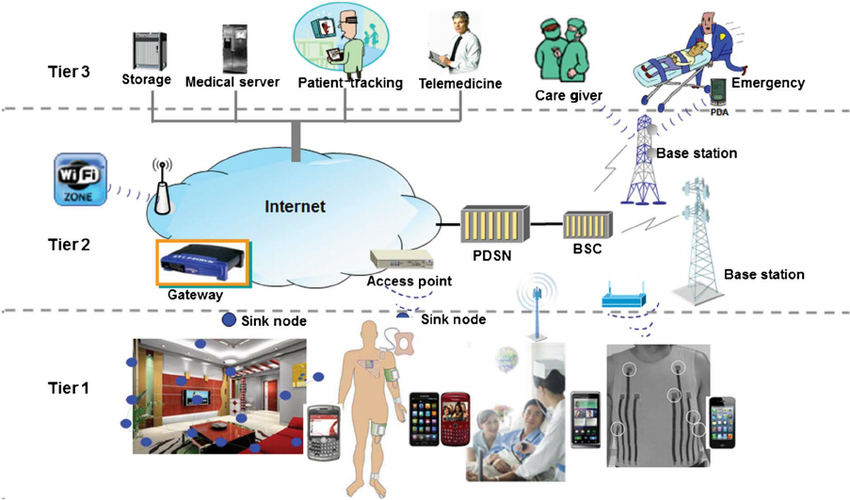
\includegraphics[scale=0.5,width=12cm,height=6.5cm]{photos/healthcare.png}
		\caption{Health Care Applications}
			\centering
		\label{fig:x Health_Care_Applications}
		\hspace*{\fill}
	\end{figure}
		
		%figure Health Care Application Right here
		%\begin{figure}[h!]
		%	\centering
		%	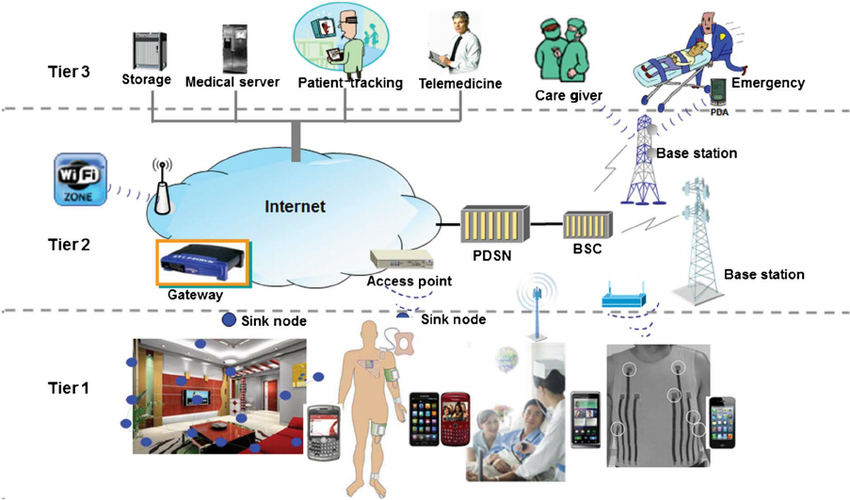
\includegraphics[scale=0.5,width=15cm,height=9cm]{photos/healthcare.png}
		%	\caption{Health Care Applications}
		%	\label{fig:x Health_Care_Applications}
			
		%\end{figure}
	
  \begin{figure}	
	\subsection{Home Intelligence}
			 Wireless sensor networks can be used to provide more convenient and intelligent living environments for human beings. For example, wireless sensors can be used to remotely read utility  meters in a home like water, gas, electricity and then  send  the  readings  to  a  remote  centre 
		through  wireless communication\cite{application} see\ref{fig:x Home_Intelligence}.
	
		\hfill
		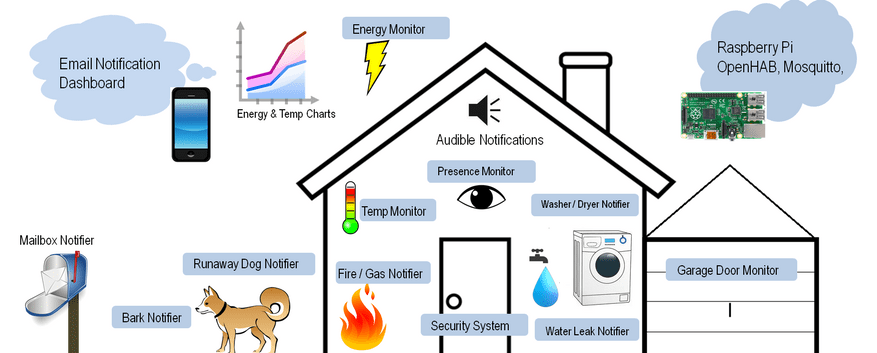
\includegraphics[scale=0.5,width=12cm,height=6.5cm]{photos/home.png}
		\caption{Home Intelligence}
		\label{fig:x Home_Intelligence}
			\centering
		\hspace*{\fill}
  \end{figure}
		  
    %figure Home Intelligence
   % \begin{figure}[h!]
    %	\centering
   % 	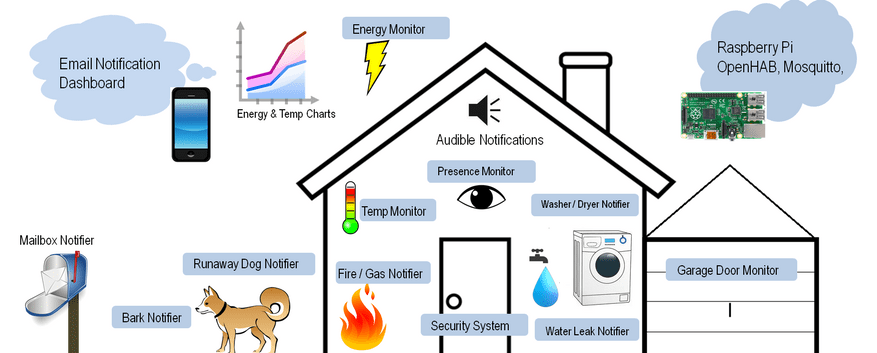
\includegraphics[scale=0.5,width=15cm,height=9cm]{photos/home.png}
    %	\caption{Home Intelligence}
    %	\label{fig:x Home_Intelligence}
    	
    % \end{figure}
    
   \begin{figure} 
    \subsection{Agriculture}
    
    Using wireless sensor networks within the agricultural industry  is  increasingly  common,  using  a  wireless  network frees the farmer from the maintenance of wiring in a difficult environment. Gravity  feed  water  systems  can  be  monitored using  pressure  transmitters  to  monitor  water  tank  levels, pumps can be controlled using wireless I/O devices and water use  can  be  measured  and  wirelessly  transmitted  back  to  a central  control  center  for  billing.  Irrigation  automation enables more efficient water use and reduces waste\cite{application} see\ref{fig:x Agriculture_}.
    
    %%figure Agriculture
	%\begin{figure}[h!]
	%	\centering
	%	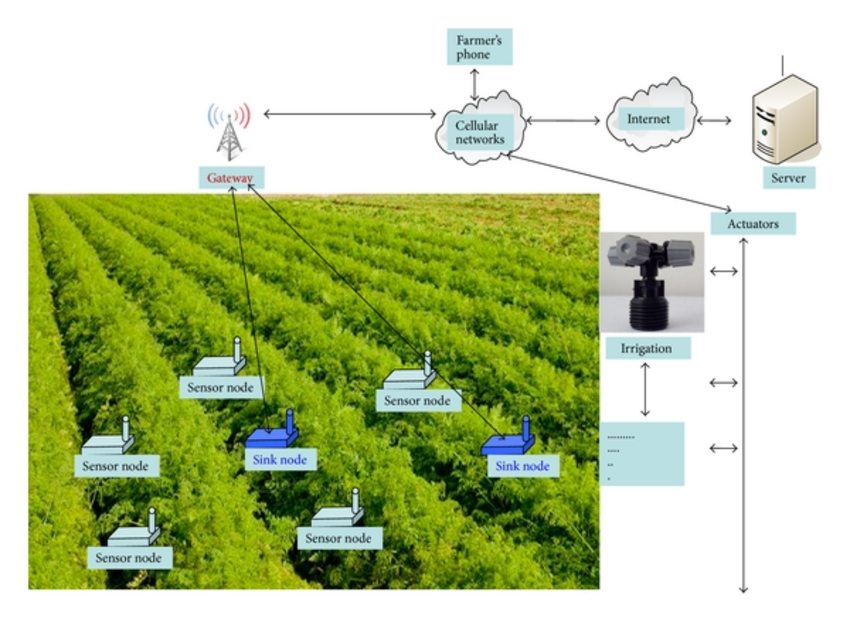
\includegraphics[scale=0.5,width=12cm,height=6cm]{photos/agri.png}
	%	\caption{Agriculture}
	%	\label{fig:x Agriculture_}
		
	%\end{figure}

	\hfill
	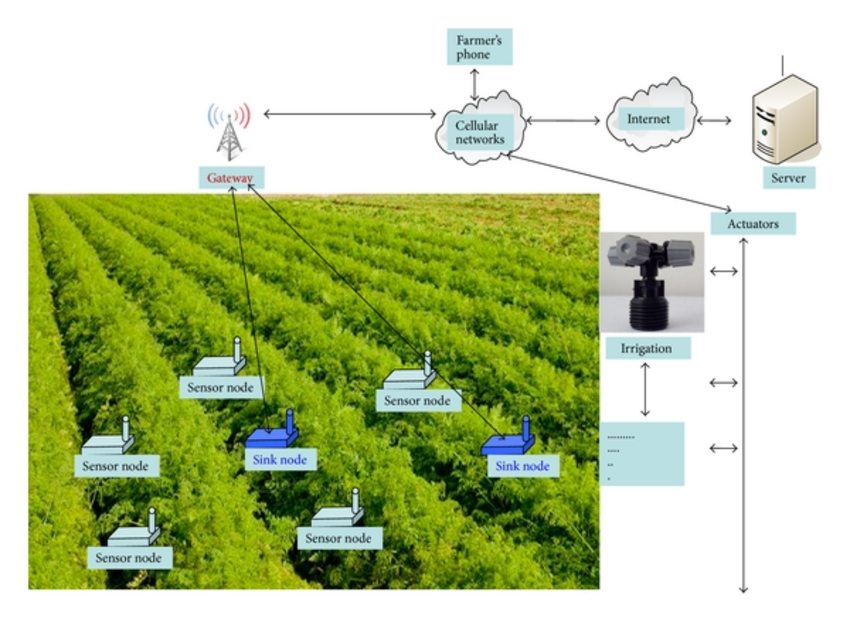
\includegraphics[scale=0.5,width=12cm,height=5cm]{photos/agri.png}
	\caption{Agriculture}
	\centering
	\label{fig:x Agriculture_}
	\hspace*{\fill}
\end{figure}
\section{Challenges}

Recent advances in technology has made researchers quite optimistic towards the feasibility of Wireless sensor networks (WSNs).  These are being deployed for various applications and have huge potential for research. However, owing to the multidisciplinary nature of this field, researchers have to face many a technical hitches,research issues and challenges involved in the design of WSNs\cite{resGateChallenges}. 
The major challenges that affect the design and performance of a wireless sensor network are as follows :
	\subsection{Energy}
	The first and  often most important design challenge for a WSN is energy efficiency.Power consumption  can  be  allocated  to  three  functional  domains: sensing, communication, and data processing, each of which requires  optimization.  The  sensor  node  lifetime  typically exhibits a  strong dependency on battery life. The constraint most  often  associated  with  sensor  network  design  is  that sensor nodes operate with limited energy budgets[ref.energy] \cite{energy}.  
	\newline
	Typically,  sensors  are  powered  through  batteries,which  must  be  either  replaced  or  recharged  when  depleted. For non rechargeable batteries, a sensor node should be able to  operate  until  either  its  mission  time  has  passed  or  the battery  can  be  replaced.  The  length  of  the  mission  time depends on the type of application\cite{energy}. 
	
	
	\subsection{Synchronization}
	Clock  synchronization is an important  service  in  sensor networks.Time Synchronization in a sensor network aims to provide a common timescale for local clocks of nodes  in  the  network.A global clock in a sensor  system  will  help  process and analyze the data  correctly and predict future system behavior.Some applications that require global clock synchronization are environment monitoring ,navigation guidance, vehicle tracking etc. A clock synchronization service for a sensor network has to meet challenges that are substantially different from those in infrastructure based networks\cite{sync2} \cite{sync1}
	
	
	
	\subsection{Security}
	Security in sensor networks is as much an important factor as performance    and    low    energy    consumption    in    many applications. Security in a sensor network is very challenging as WSN is not only being deployed in battlefield applications but  also  for  surveillance,  building  monitoring,  burglar  alarms  and in critical systems such as airports and hospitals\cite{}[Ref.security].
	Since  sensor  networks  are  still  a  developing  technology, researchers  and  developers  agree  that  their  efforts  should  be concentrated  in  developing  and  integrating  security  from  the  initial phases of sensor applications development; by doing so,they hope to provide a stronger and complete protection against illegal  activities  and  maintain  stability  of  the  systems  at  the  same time\cite{}.
	
	
	
	\subsection{Quality Of Service}
	WSNs are   becoming   more widely  deployed  for  real-world  monitoring, event detection,and target tracking  [e.g., \cite{}Ref.Qos]. Many of these applications require the  WSN  to  operate  autonomously in dynamic environmental settings, with desirable quality of service (QoS) where  the  control  is  adaptive  to  various  factors  such  as  task’s changing  requirements,network  conditions,  node  failure,  and mobility  in  real-time.  In  particular,  as  sensor  nodes  in  a WSN are typically battery-operated,any WSN QoS control  algorithms  should  be  energy-aware  and  power-efficient  to  be practical. 



	\subsection{Limited bandwidth}
	In   wireless   sensor   nets,   much   less   power   is consumed in processing data than transmitting it. Presently,wireless communication is limited to a data rate in the order of 10–100 Kbits/second.Bandwidth   limitation   directly   affects   message exchanges among sensors,and     synchronization is impossible  without  message  exchanges.  Sensor  networks often operate in a bandwidth and performance constrained multi-hop  wireless communications medium.These wireless communications links operate in the radio, infrared,or optical range[\cite{}.Ref energy].   
	
	\subsection{Node Costs}
	A  sensor  network  consists  of  a  large  set  of  sensor nodes.  It  follows  that  the  cost  of  an  individual  node  is critical to the overall financial metric of the sensor network. Clearly, the cost of each sensor node has to be kept low for the global metrics  to  be acceptable.  Depending  on  the application  of  sensor  network,  large  number  sensors  might be scattered randomly over an environment, such as weather monitoring.  If  the  overall  cost  was  appropriate  for  sensor networks  and  it  will be more acceptable and successful to users which need careful consideration[\cite{}Ref. energy]. 
	
	\subsection{Deployment}
	Node  deployment  is  a  fundamental  issue  to  be solved   in   Wireless   Sensor   Networks.   A   proper   node deployment scheme can reduce the complexity of problems.Deploying  and  managing  a  high  number  of  nodes  in  a relatively bounded environment requires special techniques. Hundreds  to  thousands  of  sensors  may  be  deployed  in  a sensor region. There are two deployment models at present:
	\paragraph{static  deployment} The  static deployment   chooses   the   best   location   according   to  the optimization  strategy,  and  the  location  of  the  sensor  nodes has  no  change  in  the lifetime of the  WSN
	 \paragraph{dynamic  deployment} The dynamic deployment throws the nodes randomly for optimization.  
	 
	 
	